\documentclass[a4paper, 10pt]{report}
\usepackage[compat=1.1.0]{tikz-feynman}

\begin{document}

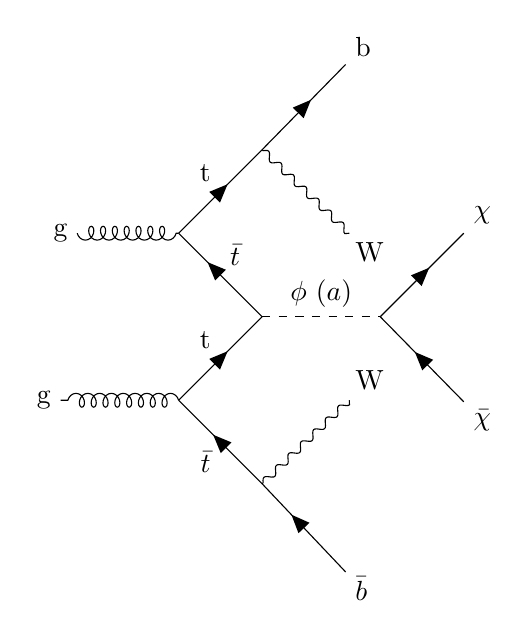
\begin{tikzpicture}[sibling distance=4cm]
  \begin{feynman}  
    \vertex (g1) {g};    
    \vertex [right=of g1] (a);
    \vertex [above right=of a] (t1);
    \vertex [above right=of t1] (b1) {b};
    \vertex [below right=of t1] (W1) {W};
    \vertex [below right=of a] (c);
    \vertex [below left=of c] (b);
    \vertex [left=of b] (g2) {g};
    \vertex [below right=of b] (t2);
    \vertex [below right=of t2] (b2) {$\bar b$};
    \vertex [above right=of t2] (W2) {W};
	\vertex [right=of c] (m);
	\vertex [above right=of m] (d1) {$\chi$};
	\vertex [below right=of m] (d2) {$\bar \chi$};
 
    \diagram* {
      (g1) -- [gluon] (a) -- [fermion, edge label={t}] (t1),
      (t1) -- [fermion] (b1),
      (t1) -- [boson] (W1),
      (a) -- [anti fermion, edge label={$\bar t$}] (c),
      (b) -- [fermion, edge label={t}] (c),
      (t2) -- [fermion, edge label={$\bar t$}] (b) -- [gluon] (g2),
      (c) -- [scalar, edge label={$\phi$ $(a)$}] (m) -- [fermion] (d1),
      (d2) -- [fermion] (m),
      (t2) -- [anti fermion] (b2),
      (t2) -- [boson] (W2),
    };
  \end{feynman}
\end{tikzpicture}

\end{document}